\section{Tool}
\label{cp6:tool}


To assist a participant locate text containing information potentially helpful to their task, we have developed a proof of concept web-browser plug-in 
that highlights text that a semantic-based technique 
identifies as relevant in the artifacts inspected by a participant.



The tool---\acs{beskar} (\underline{BE}RT ta\underline{sk}-relev\underline{a}nt text identifie\underline{r})---applies 
one of the most promising semantic-based techniques that we have explored in Chapter~\ref{ch:identifying} (i.e., \texttt{BERT})
to identify in an input artifact 10 sentences that are likely relevant to an input task. 
As a proof of concept, we do not focus on the tool's performance
and we have decided to pre-cache the output 
for the text identified by \acs{beskar} in each of the tasks and artifacts 
in our experiment. 


% \acs{beskar} highlights the text that it automatically identified as relevant 
% to a task in a web page so that a developer can more easily locate such text.



% \begin{figure}
%     \centering
%     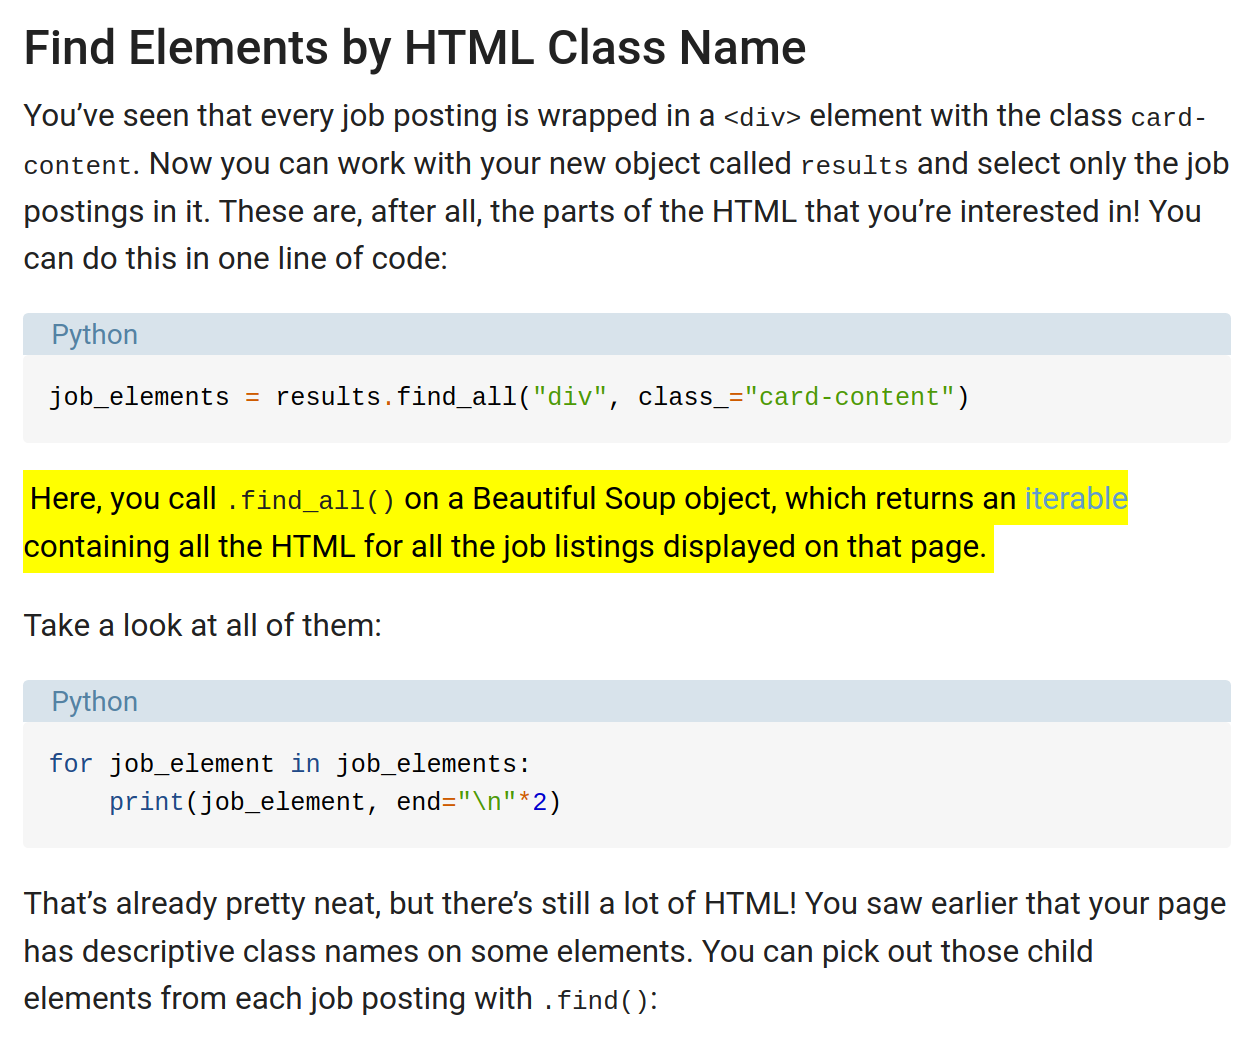
\includegraphics[width=0.85\textwidth]{cp6/tool-highlights.png}
%     \caption{Example of a highlight (in yellow) automatically identified by \acs{beskar}
%     in a web tutorial pertinent to the NYTimes task}
%     \label{fig:tool-output}
% \end{figure}

